\documentclass[a4paper]{article}
\usepackage[italian]{babel}
\usepackage[left=2cm, right=2cm, bottom=2cm, top=2cm]{geometry}
\usepackage{csvsimple}
\usepackage[utf8]{inputenc}
\usepackage{float}
\usepackage{pdfpages}
\usepackage[scaled]{helvet}
\renewcommand\familydefault{\sfdefault} 
\usepackage{pgfplots}
\usepackage{pdflscape}
%opening
\title{Relazione laboratorio Algoritmi Avanzati}
\author{Magarotto Francesco\\Muraro Enrico\\Piva Giulio}

\begin{document}
\begin{titlepage}
  \vspace*{5cm}
  \begin{center}
    \Large\bfseries
    Relazione di laboratorio
  \end{center}
  \begin{center}
    \large
    Corso di Algoritmi Avanzati\\
    Laurea Magistrale in Informatica\\A.A. 2019-2020
  \end{center}
  \vspace{4cm plus 1fill}
  \begin{flushleft}
    \large
    Magarotto Francesco - 1236594\\Muraro Enrico - 1238899 \\Piva Giulio - 1242455
  \end{flushleft}
\end{titlepage}
\newpage

\section{Introduzione}

è valutare le prestazioni dell'algoritmo di Karger per il problema del minimum cut rispetto a quattro parametri:
\begin{itemize}
\item Il tempo impiegato dalla procedura di Full Contraction
\item Il tempo impiegato dall'algoritmo completo per ripetere la contrazione un numero sufficientemente alto di volte
\item Il discovery time, ossia il momento in cui l'algoritmo trova per la prima volta il taglio di costo mimimo
\item L'errore nella soluzione trovata rispetto al risultato ottimo
\end{itemize}
Il linguaggio di programmazione scelto dal nostro gruppo è Java.

\subsection{Esecuzione del programma}
Gli algoritmi sono stati sviluppati come progetto Maven. All'interno della cartella \'e presente la versione portable di Maven, pertanto non è necessario averlo installato. \'E
richiesto almeno il JDK 11 installato nel sistema.
Per eseguire i tre algoritmi utilizzare i seguenti comandi:\\
Linux:\\
\indent \texttt{./mvnw install}\\
\indent \texttt{./mvnw exec:java}\\
Windows:\\
\indent \texttt{mvnw.cmd install}\\
\indent \texttt{mvnw.cmd exec:java}

L'esecuzione del main genera automaticamente dei file csv nella directory del progetto contenenti i tempi registrati. L'algoritmo di Karger viene interrotto dopo 60 secondi.
\subsection{Strutture dati utilizzate}

Per rappresentare il grafo abbiamo utilizzato una matrice di adiacenza visto che i sono grafi completi e la matrice viene quindi riempita senza sprechi di memoria.

Nell'algoritmo 2 Approssimato abbiamo fatto uso di un HashMap per registrare la visita in preordine del grafo.

La classe Heap è una nostra implementazione di MinHeap. L'albero binario è rappresentato da un array di interi, i valori all'interno dell'array corrispondono ai nodi presenti nel grafo. Il confronto tra i nodi per determinare il più piccolo è effettuato tramite un Comparator passato alla creazione dello Heap, questo per avere un'implementazione di Heap indipendente dal modo in cui viene utilizzato da uno specifico algoritmo.
\subsection{Lettura di un grafo da file}
Per caricare un grafo in memoria, abbiamo implementato una classe GraphReader, che si occupa della lettura del file tramite la libreria \textit{nio} di Java. Inoltre effettua le conversioni di distanza necessarie sia per i file di tipo GEO che EUC\_2D e ritorna direttamente la matrice di adiacenza del grafo.


\subsection{Implementazione di Held-Karp}

L'algoritmo di Held-Karp necessita di due strutture di supporto, una per salvare le distanze minime già calcolate e una per ricordare il nodo precedente in modo da poter ricostruire il percoso trovato. Visto che entrambi sono identificati da due valori (v,S) dove 'v' è un nodo e 'S' un insieme di nodi abbiamo deciso di implementare entrambe con ArrayList di HashMap. Ogni posizione dell'ArrayList corrisponde a un nodo e contiene una mappa che ha come chiave un Set di nodi. In questo modo con due accessi costanti possiamo trovare il valore desiderato.

Il timeout di Held-Karp è controllato da un flag booleano, quando viene impostato il valore del flag a 'true' il ciclo che cerca il minimo viene interrotto e l'algoritmo ritorna la soluzione migliore trovata fino a quel momento.

Quando eseguiamo l'algoritmo facciamo quindi partire un thread usando ScheduledExecutorService, che dopo 5 minuti imposta il flag a 'true' terminando l'esecuzione.

\subsection{Implementazione dell'euristica nearest-neighbor}
L'Euristica nearest-neighbor consiste nel trovare il prossimo vertice, non ancora inserito nel circuito, a distanza minima dal nodo corrente. Una volta visitati tutti i nodi
ripetendo questa operazione si otter\'a un percordo 2-approssimato per il problema del TSP. Questa euristica \'e di facile implementazione, ma allo stesso tempo molto efficace.

\subsection{Implementazione dell'algoritmo 2-approssimato}
L'algoritmo 2-approssimato \'e basato su una tecnica molto semplice: Si trova un MST con l'algoritmo di Prim e poi si visita l'albero in ordine prefisso.
Nel nostro caso, Prim restituisce il MST sotto forma di HashMap, dove la chiave \'e un nodo e il value la lista dei suoi figli. A questo punto l'albero viene visitato in ordine
prefisso dal metodo Preorder, restituendo un percorso approssimato per il problema del TSP.
\section{Risultati ottenuti}
\begin{figure}[H]
	\centering
	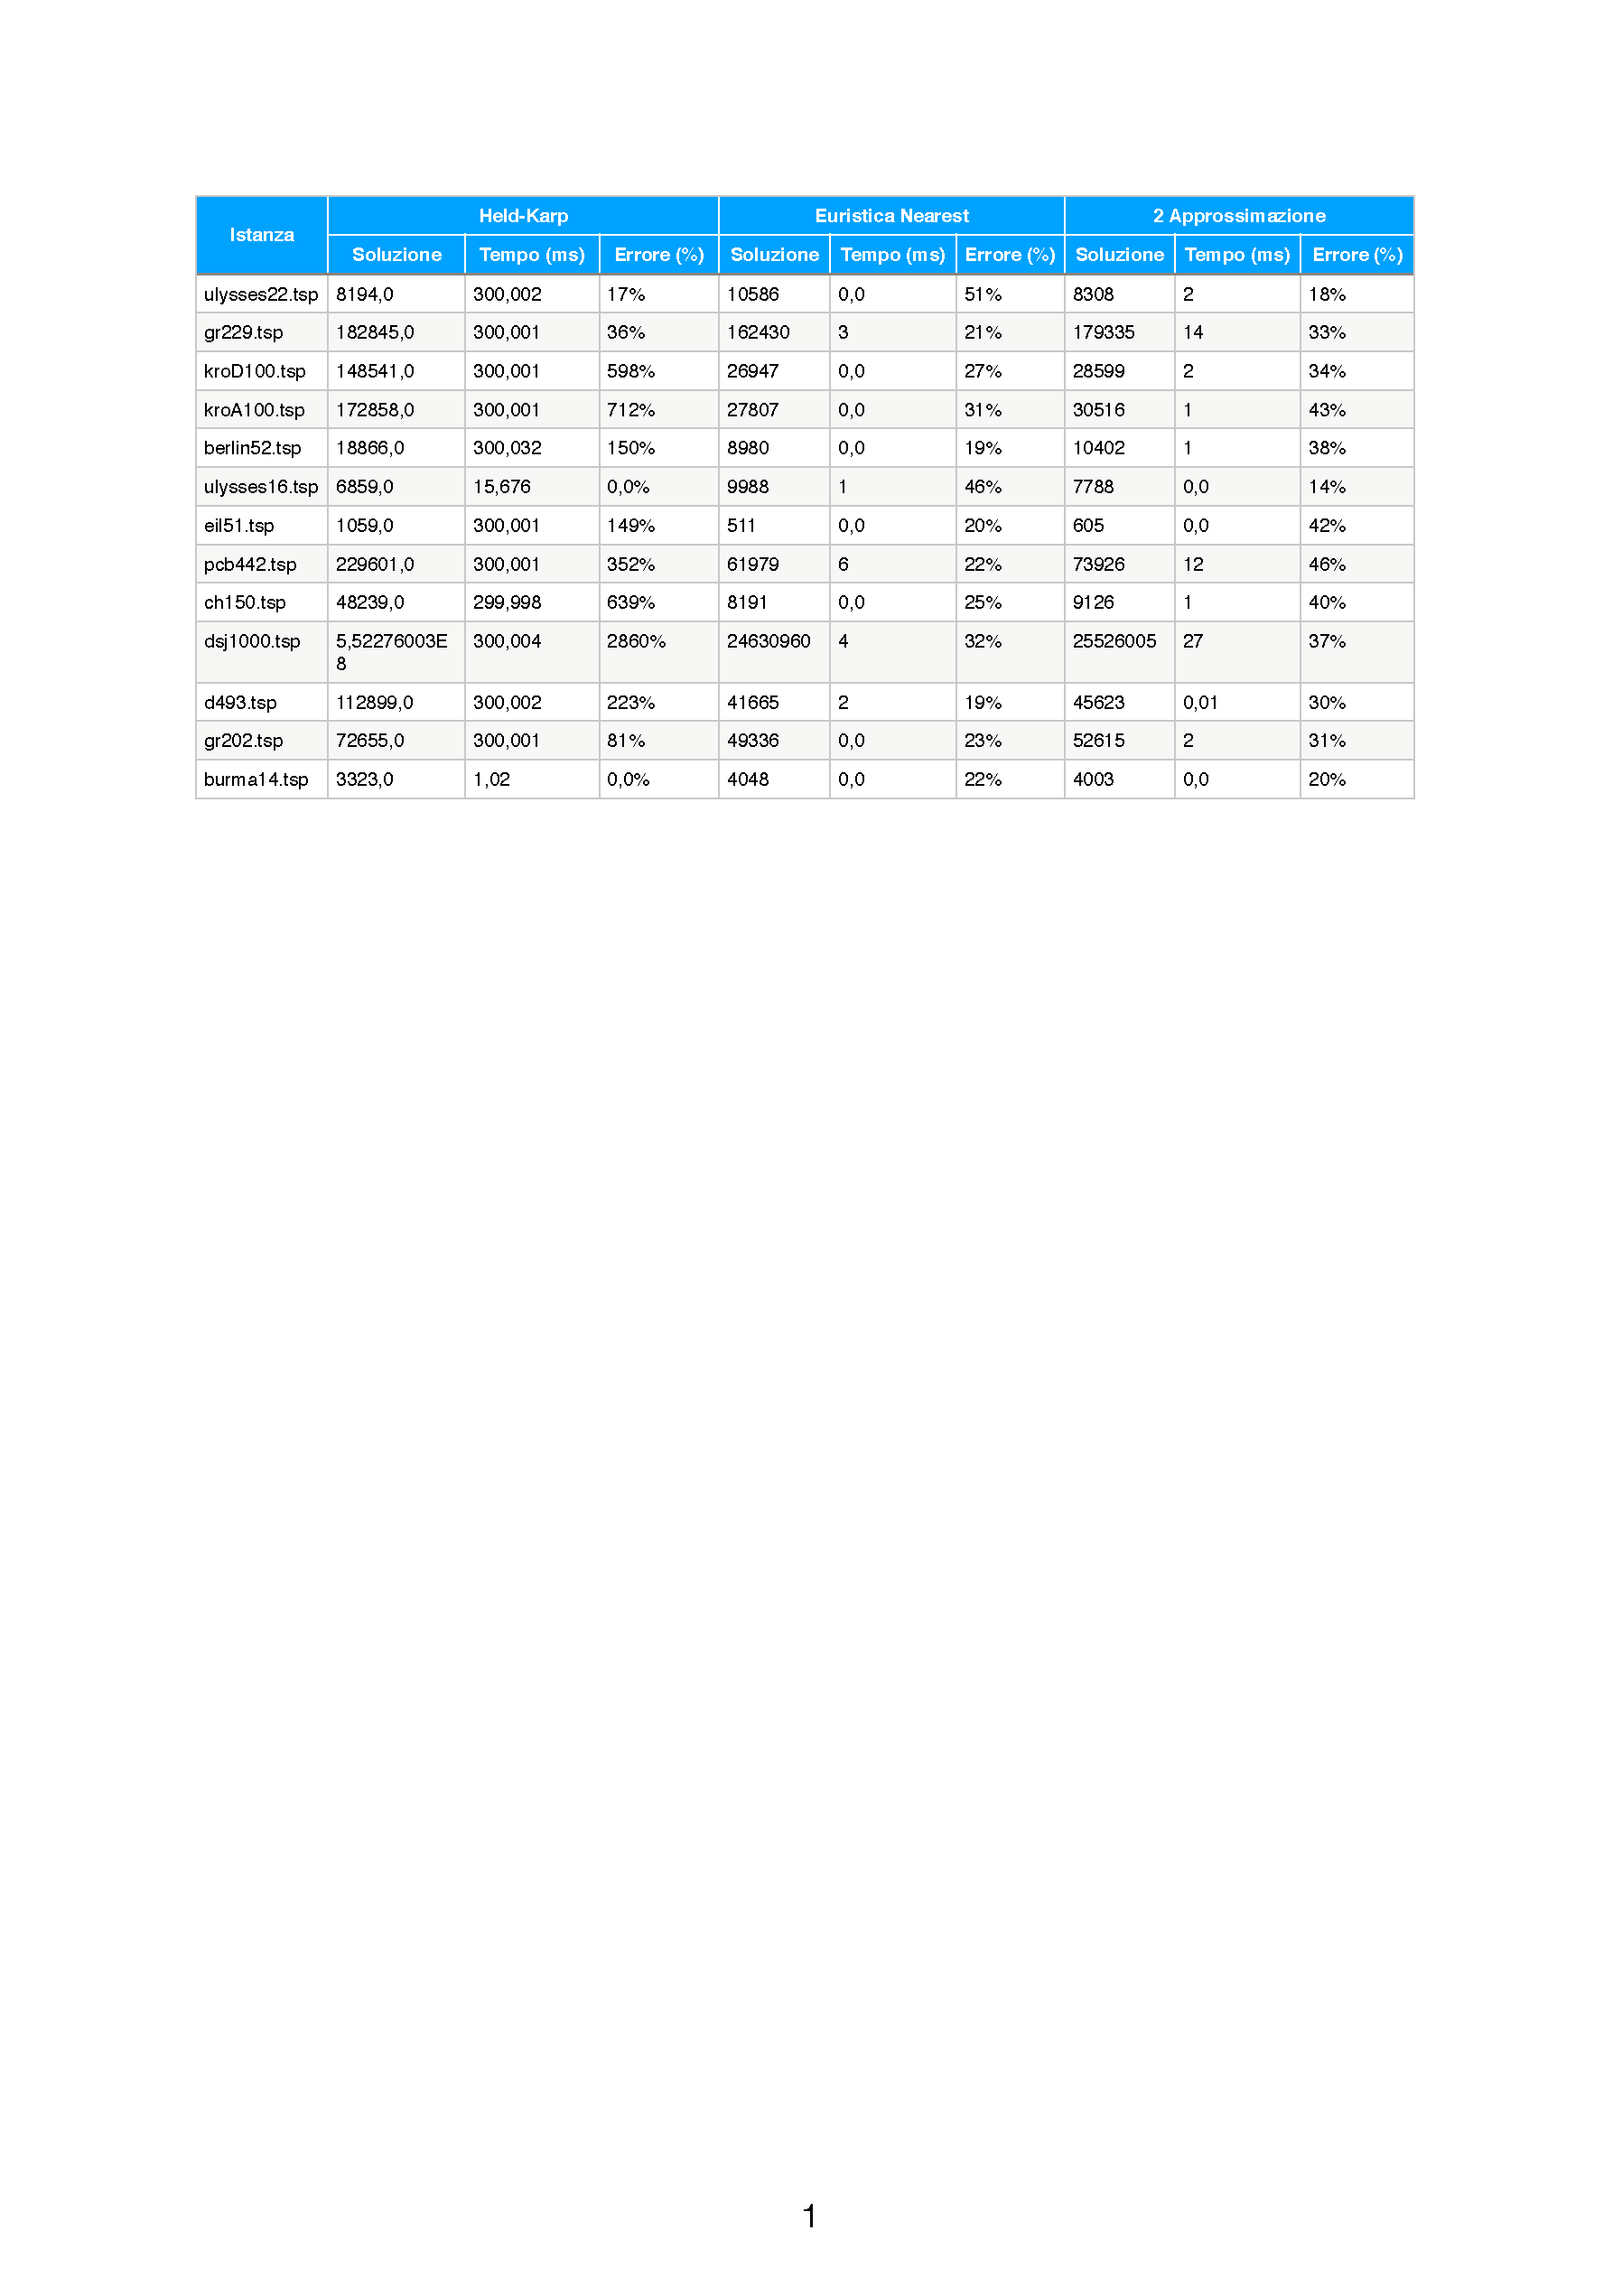
\includegraphics[width=17cm]{tabellapdf}
\end{figure}
Come possiamo vedere dalla tabella, nell'algoritmo di Held-Karp solo poche istanze \textbf{non} sono andate in \textit{timeout}. Infatti, i grafi con tempo di esecuzione maggiore di circa 300000 secondi, sono state interrotte. Pertanto l'83.3\% delle esecuzioni dell'algoritmo di Held-Karp ritorna la soluzione calcolata fino a quel momento, con un conseguente tasso di errore molto alto, anche del 2860\% come nel caso dell'istanza \texttt{dsj1000.tsp}.

\begin{figure}[H]
	\centering
	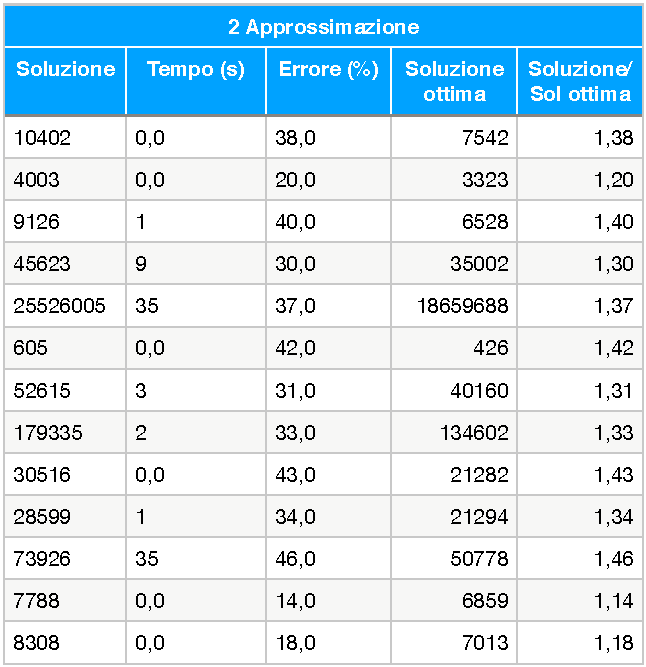
\includegraphics[width=0.5\linewidth]{2approx}
	\label{fig:2approx}
\end{figure}
Questa tabella invece mostra l'approssimazione calcolata dall'algoritmo è 2 approssimata. Infatti,
$\frac{Soluzione}{Solzione\ ottima} = \rho(p) \leq 2$
\begin{figure}[H]
	\begin{center}
	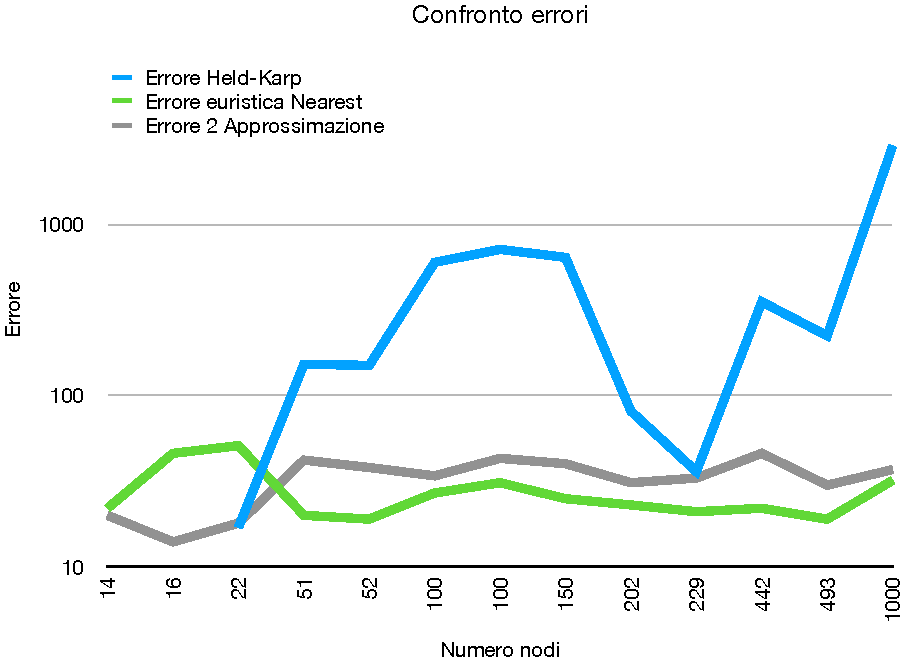
\includegraphics[width=17cm]{errore}
	\caption{Istogramma che mette in relazione gli errori dei tre algoritmi utilizzando la scala logaritmica. Come era prevedibile dalla tabella sopra, l'errore maggiore è presente nell'algoritmo di Held-Karp, che in questi pochi esempi non è sempre crescente poiché il numero di istanze è esiguo. Certamente con un numero di maggiore di nodi, avremmo due possibili scenari: mantenendo lo stesso tempo massimo di esecuzione, l'errore sarebbe molto alto, mentre aumentando il tempo di esecuzione, lo stack verrebbe riempito delle chiamate ricorsive, portando ad un'eccezione runtime OutOfMemory.}	\label{fig:errore}
\end{center}
\end{figure}

\subsubsection{Tempo di timeout Held-Karp}
Abbiamo provato varie esecuzioni dell'algoritmo di Held-Karp per verificare come varia l'errore in relazione al raddoppio del tempo prima del timeout.
\begin{figure}[H]
	\centering
	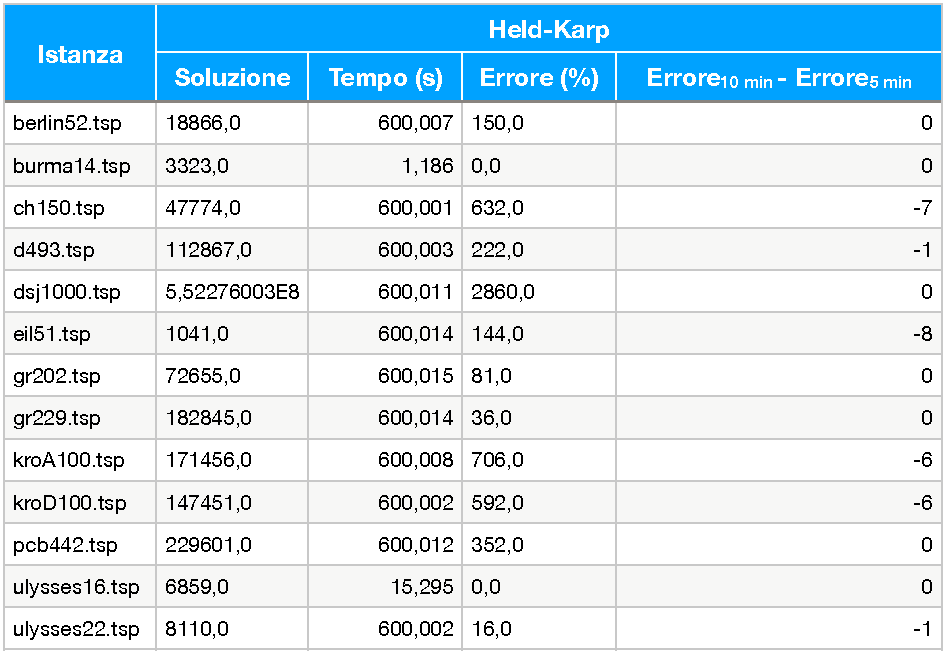
\includegraphics[width=0.5\linewidth]{differenze_errori}
	\label{fig:timeouttiming}
	\caption{Tabella che mostra come l'errore sia variato in relazione all'aumento del tempo di esecuzione dell'algoritmo. In particolare, aumentando il tempo prima del timeout da 5 a 10 minuti, solo i grafi di dimensione compresa tra 20 e 100 hanno avuto un beneficio. I grafi con un numero di nodi superiore a 200 \textbf{non} hanno avuto alcun beneficio dall'aumento del tempo di esecuzione.}
\end{figure}

\section{Conclusioni}
L'algoritmo migliore tra i tre è l'euristica Nearest che presenta un tasso di errore minore, avvicinandosi di più alla soluzione ottima. La soluzione dell'euristica Nearest Neighbor è $O(log(n))$ - approssimata a TSP, quando la disuguaglianza triangolare è rispettata. La complessità Held-Karp con table filling ha complessità $O(n^2*2^n)$, che è esponenziale e interropendo l'esecuzione a 5 minuti non permette .
\end{document}
